\documentclass[12pt,a4paper]{article}
\usepackage[T1]{fontenc}
\usepackage[utf8]{inputenc}
\usepackage[polish]{babel}
\usepackage{graphicx}
\usepackage{listings}
\usepackage{xcolor}
\usepackage{hyperref}
\usepackage{geometry}
\usepackage{enumitem}
\usepackage{float}

\geometry{
    a4paper,
    total={170mm,257mm},
    left=20mm,
    top=20mm,
}

\definecolor{codegreen}{rgb}{0,0.6,0}
\definecolor{codegray}{rgb}{0.5,0.5,0.5}
\definecolor{codepurple}{rgb}{0.58,0,0.82}
\definecolor{backcolour}{rgb}{0.95,0.95,0.92}

\lstdefinestyle{mystyle}{
    backgroundcolor=\color{backcolour},   
    commentstyle=\color{codegreen},
    keywordstyle=\color{magenta},
    numberstyle=\tiny\color{codegray},
    stringstyle=\color{codepurple},
    basicstyle=\tiny\ttfamily,
    breakatwhitespace=false,
    breaklines=true,
    captionpos=b,
    keepspaces=true,
    numbers=left,
    numbersep=5pt,
    showspaces=false,
    showstringspaces=false,
    showtabs=false,
    tabsize=2
}

\lstset{style=mystyle}

\lstdefinelanguage{JavaScript}{
  keywords={async, const, let, var, function, return, if, else, for, while, do, switch, case, break, continue, new, try, catch, throw, typeof, instanceof},
  keywordstyle=\color{magenta}\bfseries,
  ndkeywords={class, export, boolean, throw, implements, import, this, await},
  ndkeywordstyle=\color{blue}\bfseries,
  identifierstyle=\color{black},
  sensitive=false,
  comment=[l]{//},
  morecomment=[s]{/*}{*/},
  commentstyle=\color{codegreen}\ttfamily,
  stringstyle=\color{codepurple}\ttfamily,
  morestring=[b]',
  morestring=[b]",
  basicstyle=\tiny\ttfamily,
  literate=%
    {ą}{{\k{a}}}1
    {ć}{{\'c}}1
    {ę}{{\k{e}}}1
    {ł}{{\l{}}}1
    {ń}{{\'n}}1
    {ó}{{\'o}}1
    {ś}{{\'s}}1
    {ż}{{\.z}}1
    {ź}{{\'z}}1
    {Ą}{{\k{A}}}1
    {Ć}{{\'C}}1
    {Ę}{{\k{E}}}1
    {Ł}{{\L{}}}1
    {Ń}{{\'N}}1
    {Ó}{{\'O}}1
    {Ś}{{\'S}}1
    {Ż}{{\.Z}}1
    {Ź}{{\'Z}}1
}

\begin{document}
\begin{titlepage}
    \begin{center}
        \vspace*{2cm}
        {\huge\bfseries Prezentacja sterowana gestami\par}
        \vspace{1.5cm}
        {\Large\itshape Dokumentacja Projektowa\par}
        \vspace{1.5cm}
        {\large Autor:\par}
        {\large\bfseries Filip Kula, Wiktor Mazur\par}
        \vspace{1cm}
        {\large Przedmiot:\par}
        {\large\itshape Interakcja Człowiek - Komputer\par}
    \end{center}
\end{titlepage}

\newpage

\section{Wprowadzenie}

Celem systemu jest zapewnienie interaktywnego sposobu zarządzania prezentacją bez konieczności użycia myszy lub klawiatury. Dzięki zastosowaniu technologii rozpoznawania gestów użytkownik może płynnie sterować slajdami i wykonywać na nich adnotacje.

\section{Technologie}

System został zbudowany w oparciu o następujące technologie:
\begin{itemize}
    \item Next.js - framework do budowy aplikacji webowych,
    \item MediaPipe Hands - biblioteka do rozpoznawania gestów dłoni,
    \item Kontekst Canvas API - umożliwia rysowanie na slajdach,
    \item WebSocket - umożliwia komunikację w czasie rzeczywistym,
    \item Tailwind CSS - zapewnia estetyczny interfejs użytkownika.
\end{itemize}

\section{Funkcjonalności}

\subsection{Zarządzanie slajdami}
System umożliwia:
\begin{itemize}
    \item Dodawanie nowych slajdów,
    \item Usuwanie istniejących slajdów,
    \item Nawigację między slajdami za pomocą gestów dłoni.
\end{itemize}

\subsection{Obsługa gestów}
Do sterowania prezentacją wykorzystano następujące gesty:
\begin{itemize}
    \item Wskazanie w prawo - następny slajd,
    \begin{figure}[H]
      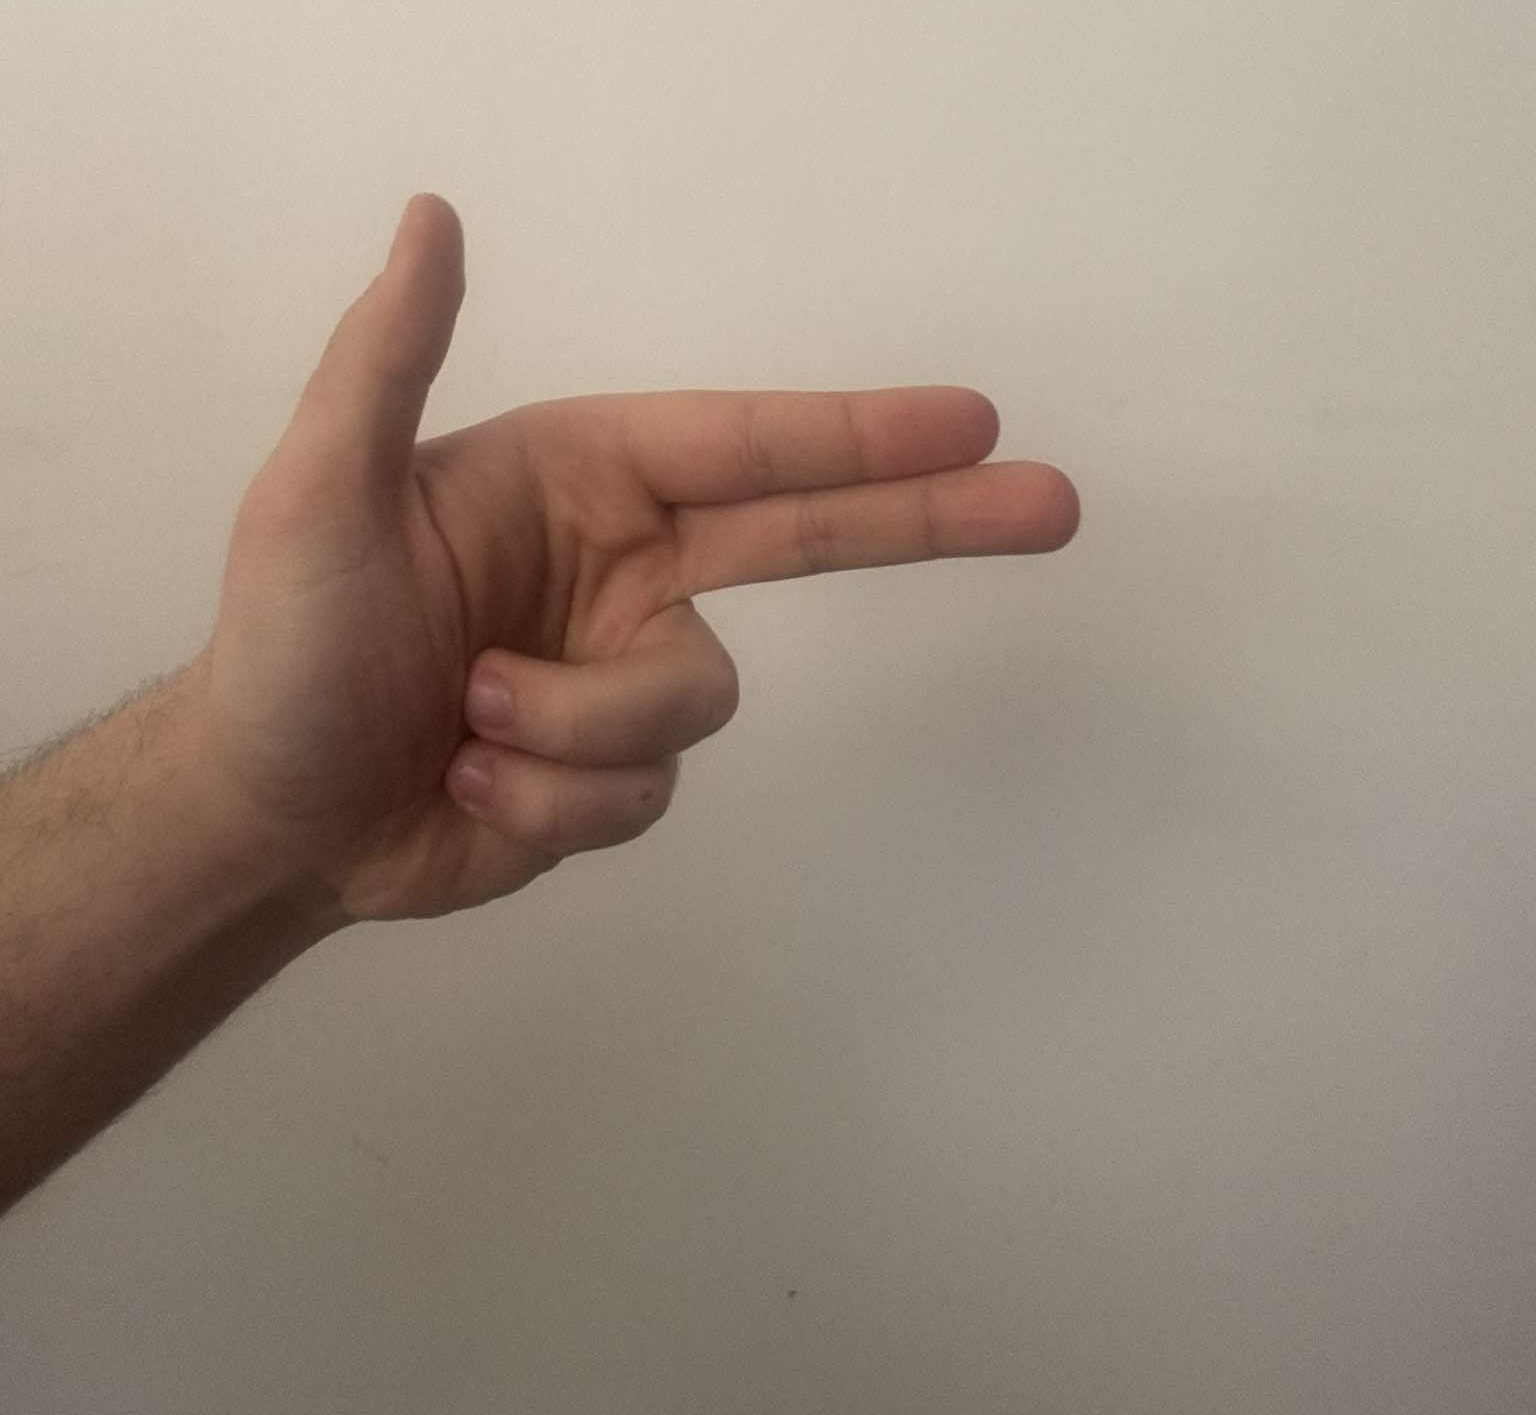
\includegraphics[width=\textwidth]{images/prawo.jpg}
    \end{figure}
    \item Wskazanie w lewo - poprzedni slajd,
    \begin{figure}[H]
      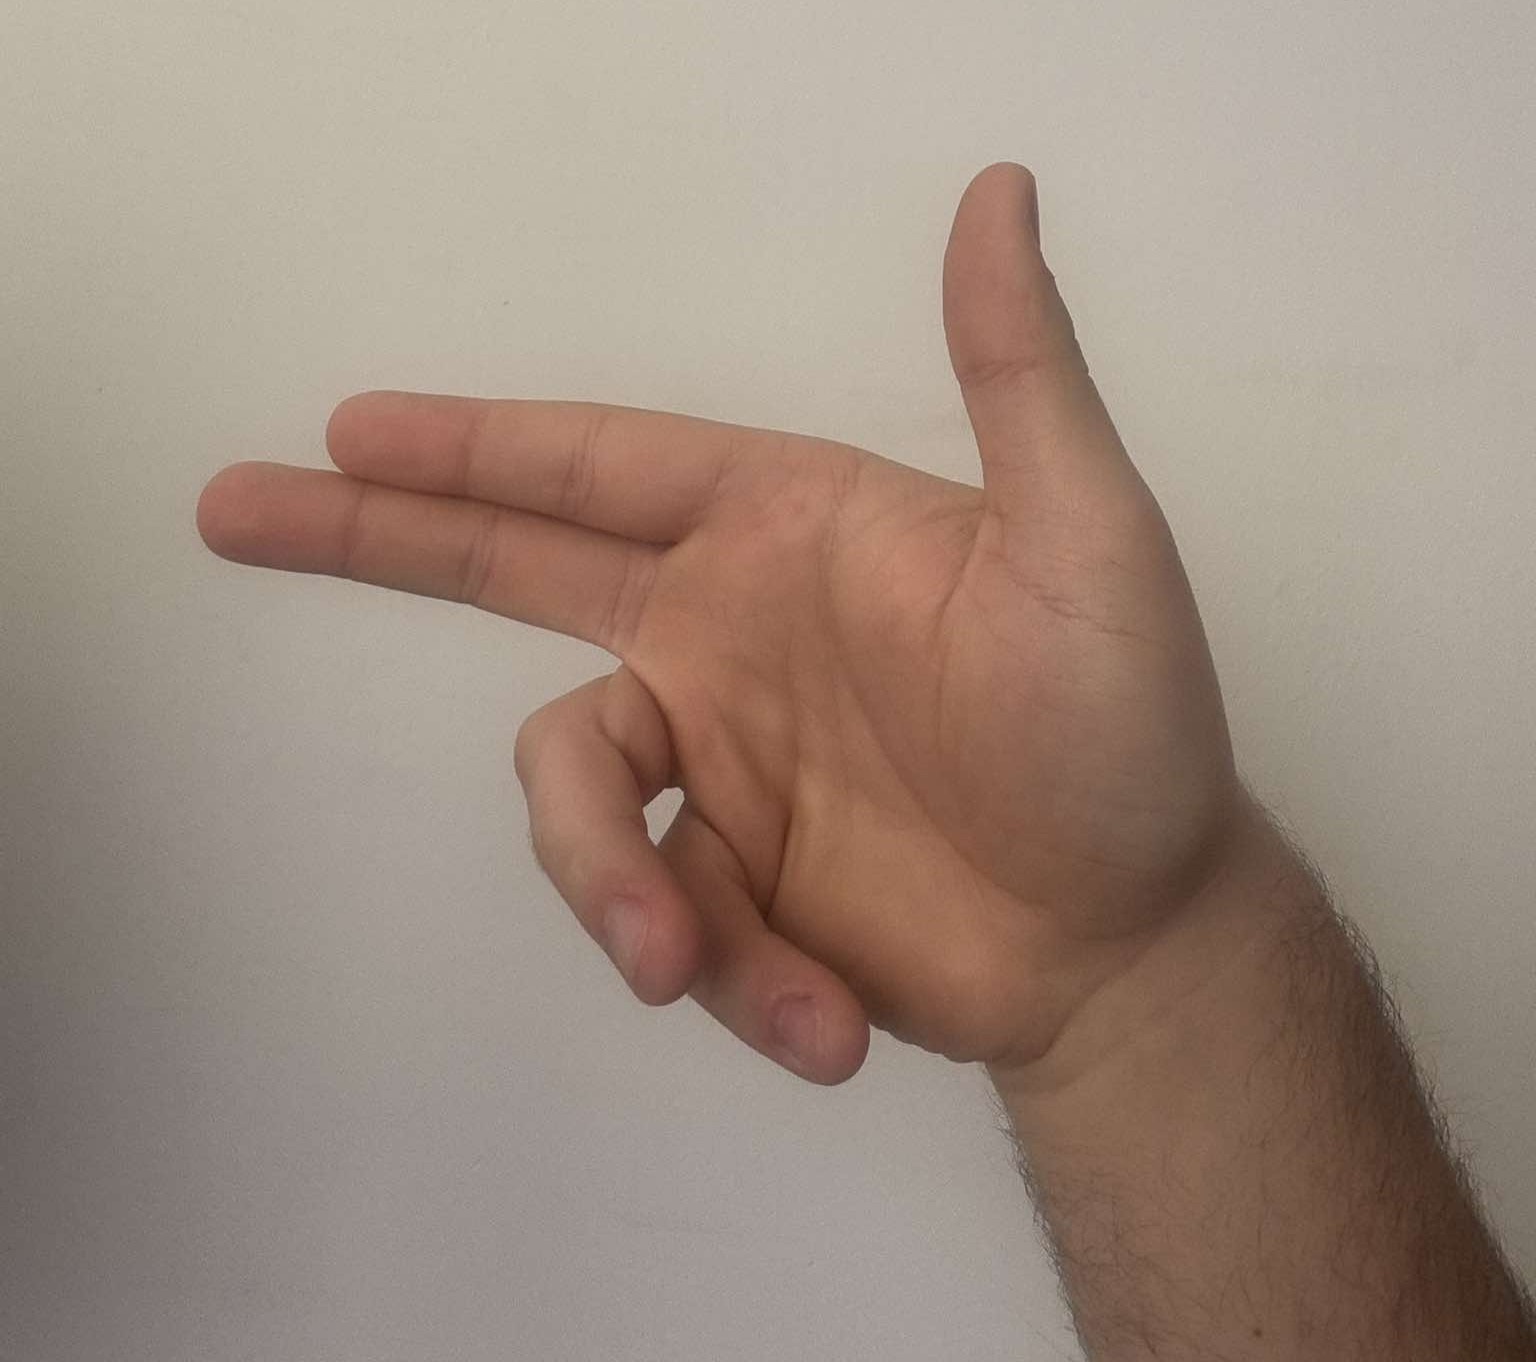
\includegraphics[width=\textwidth]{images/lewo.jpg}
    \end{figure}
    \item Zaciśnięta pięść - zmiana narzędzi.
    \begin{figure}[H]
      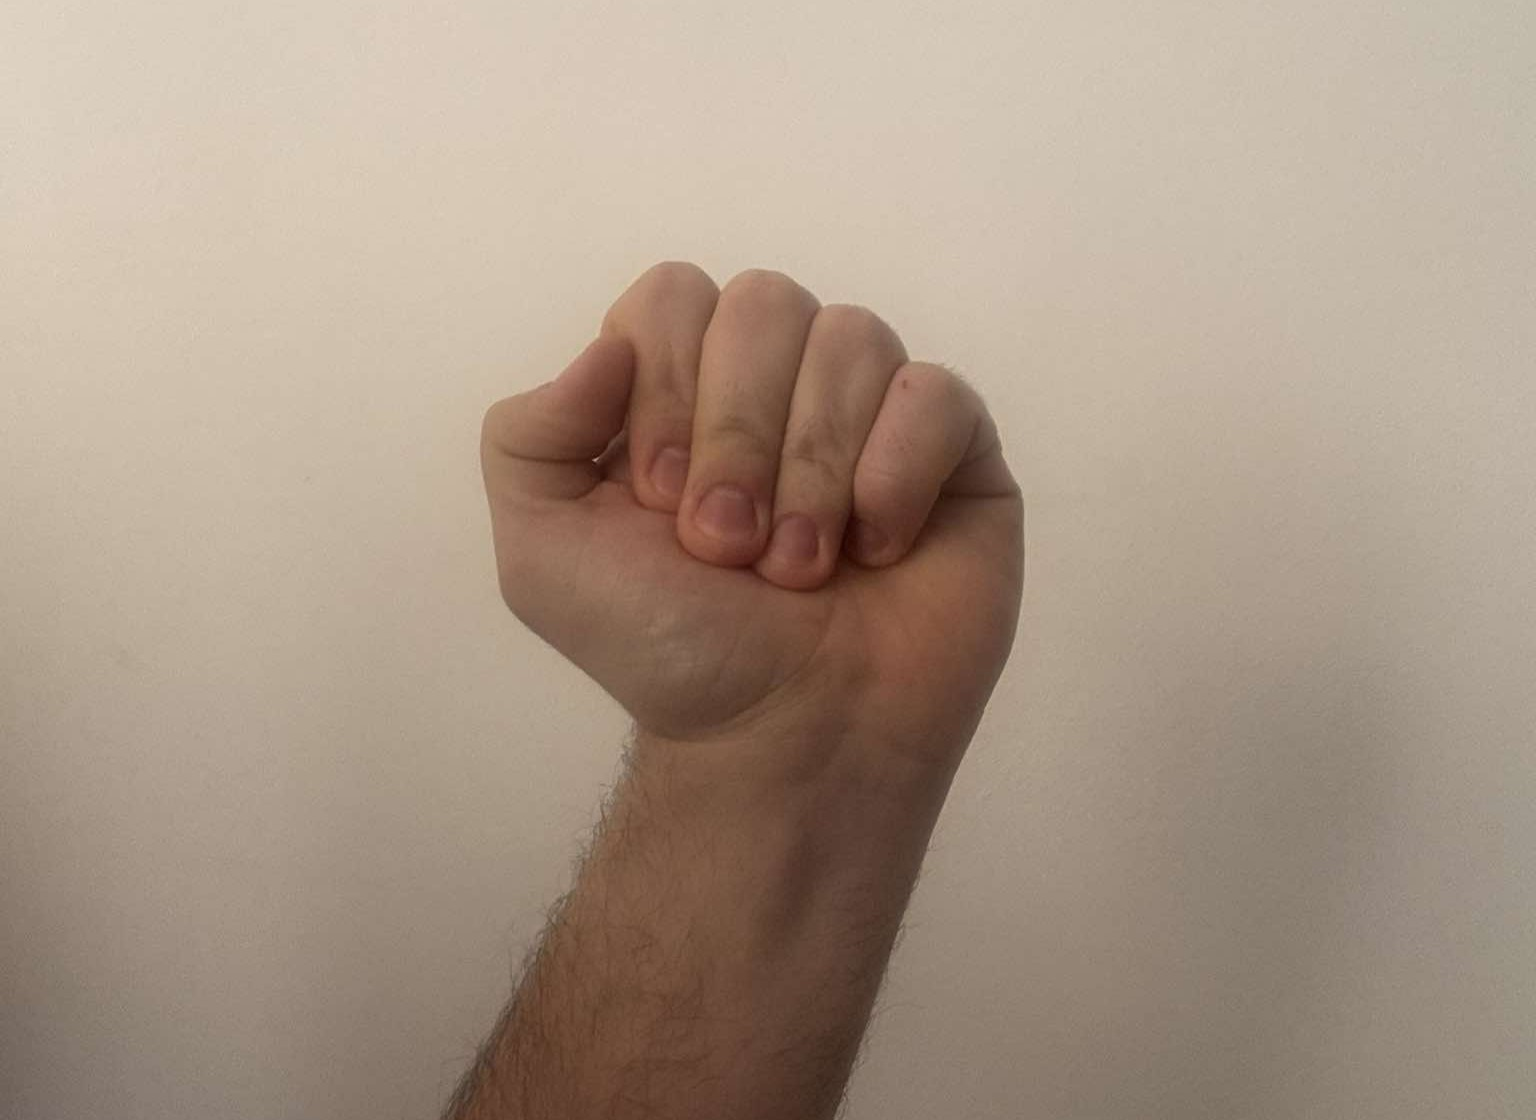
\includegraphics[width=\textwidth]{images/piesc.jpg}
    \end{figure}
\end{itemize}

\subsection{Narzędzia do rysowania}
Dostępne są następujące narzędzia:
\begin{itemize}
    \item Ołówek - rysowanie po slajdach,
    \item Gumka - usuwanie rysunków,
    \item Wskaźnik laserowy - podkreślanie elementów prezentacji.
\end{itemize}
\section{Implementacja}
\subsection{Detekcja gestów}
\begin{lstlisting}[language=JavaScript]
const detectGesture = (landmarks) => {
  if (!landmarks || landmarks.length === 0) return null;

  const hand = landmarks[0];
  const wrist = hand[0];
  const thumbTip = hand[4];
  const indexTip = hand[8];
  const middleTip = hand[12];
  
   // Wykrywanie gestu wskazywania
  const isPointing = 
    indexTip.y < middleTip.y && 
    Math.abs(thumbTip.y - wrist.y) < 0.1;

    // Wykrywanie gestu pieści
  const isFist = indexTip.y > wrist.y - 0.1;

  if (isPointing) {
    return {
      type: 'pointing',
      position: { x: indexTip.x, y: indexTip.y }
    };
  }
  if (isFist) return 'fist';
  
  return null;
};
\end{lstlisting}

\subsection{Wymagania programowe}
\begin{itemize}
    \item Nowoczesna przeglądarka internetowa (Chrome 88+, Firefox 85+, Safari 14+)
    \item Obsługa WebGL dla MediaPipe
    \item Włączona obsługa JavaScript
    \item Dostęp do kamery internetowej
    \item Minimalna rozdzielczość kamery: 640x480
    \item Stabilne połączenie internetowe (dla ładowania modeli MediaPipe)
\end{itemize}

\section{Instalacja i uruchomienie}

\subsection{Za pomocą Docker}
1. Pobierz najnowszą wersję obrazu Dockera z repozytorium na GitHubie:
\url{https://github.com/ZegarekPL/Gesture-Controlled-Presentation-Tool---Frontend/releases}

2. Załaduj obraz do Dockera:
\begin{lstlisting}[language=bash]
    docker load -i gesture_controlled_presentation_tool_frontend-v0.1.1.tar
\end{lstlisting}

3. Uruchom kontener:
\begin{lstlisting}[language=bash]
    docker run -d -p 3000:3000 gesture_controlled_presentation_tool_frontend:v0.1.1
\end{lstlisting}

4. Aplikacja będzie dostępna pod adresem: \url{http://localhost:3000}

\subsection{Instalacja lokalna}
\subsubsection{Wymagania}
\begin{itemize}
    \item Node.js 18+ 
    \item npm lub yarn
    \item Git
\end{itemize}

\subsubsection{Kroki instalacji}
1. Sklonuj repozytorium:
\begin{lstlisting}[language=bash]
git clone https://github.com/ZegarekPL/Gesture-Controlled-Presentation-Tool---Frontend.git
cd Gesture-Controlled-Presentation-Tool---Frontend
\end{lstlisting}

2. Zainstaluj zależności:
\begin{lstlisting}[language=bash]
npm install
# lub
yarn install
\end{lstlisting}

3. Uruchom aplikację w trybie deweloperskim:
\begin{lstlisting}[language=bash]
npm run dev
# lub
yarn dev
\end{lstlisting}

\end{document}